\documentclass[a4paper]{extarticle}
\usepackage{ctex}
\usepackage{titlesec}
\usepackage{lipsum}
\usepackage{geometry}
\usepackage{amsmath}
\usepackage{biblatex}
\usepackage{booktabs}
\usepackage{caption}
\usepackage{graphicx}
\usepackage{float}
\setCJKmainfont{STSong}[AutoFakeBold,AutoFakeSlant]
\setCJKsansfont{Microsoft YaHei}
\setCJKmonofont{KaiTi}
\setmainfont{Times New Roman}
\setsansfont{Times New Roman}
\setmonofont{Times New Roman}
\linespread{1.5}
\setlength{\parindent}{0pt}
\titleformat{\section}{\bfseries\fontsize{14pt}{\baselineskip}\selectfont}{\thesection}{0.5em}{}
\titleformat{\subsection}{\bfseries\fontsize{10.5pt}{\baselineskip}\selectfont}{\thesubsection}{0.5em}{}
\titleformat{\subsubsection}{\fontsize{10.5pt}{\baselineskip}\selectfont}{\thesubsubsection}{0.5em}{}
\geometry{left=2.5cm,right=2.5cm,top=2.5cm,bottom=2.5cm}
\everymath{\displaystyle}
\addbibresource{ref1.bib}

\begin{document}
    \begin{center}
        \textbf{\fontsize{22pt}{\baselineskip} \selectfont 光电效应数据处理}\\
        \vspace{2em}
        \texttt{\fontsize{14pt}{\baselineskip} \selectfont 作者:刘子墨,学号:PB23000233}\\
    \end{center}
    \section{遏止电压法测普朗克常数$h$}
    \subsection{零电流法}
    使用孔径 4 mm 的光阑,改变滤波片,测得遏止电压值如下:
    \begin{table}[H]
        \centering
        \caption{零电流法测量遏止电压值与频率的关系}
        \begin{tabular}{ccc}
            \toprule
            波长$\lambda$ (nm) & 频率 $\nu$ ($\times10^{14}$ Hz) & 遏止电压 $U_0$ (V)\\
            \midrule
            577.0 & 5.196 & 0.570\\
            546.1 & 5.490 & 0.708\\
            435.8 & 6.879 & 1.266\\
            404.7 & 7.408 & 1.558\\
            365.0 & 8.214 & 1.816\\
            \bottomrule
        \end{tabular}
    \end{table}
    拟合图像如下:
    \begin{figure}[H]
        \centering
        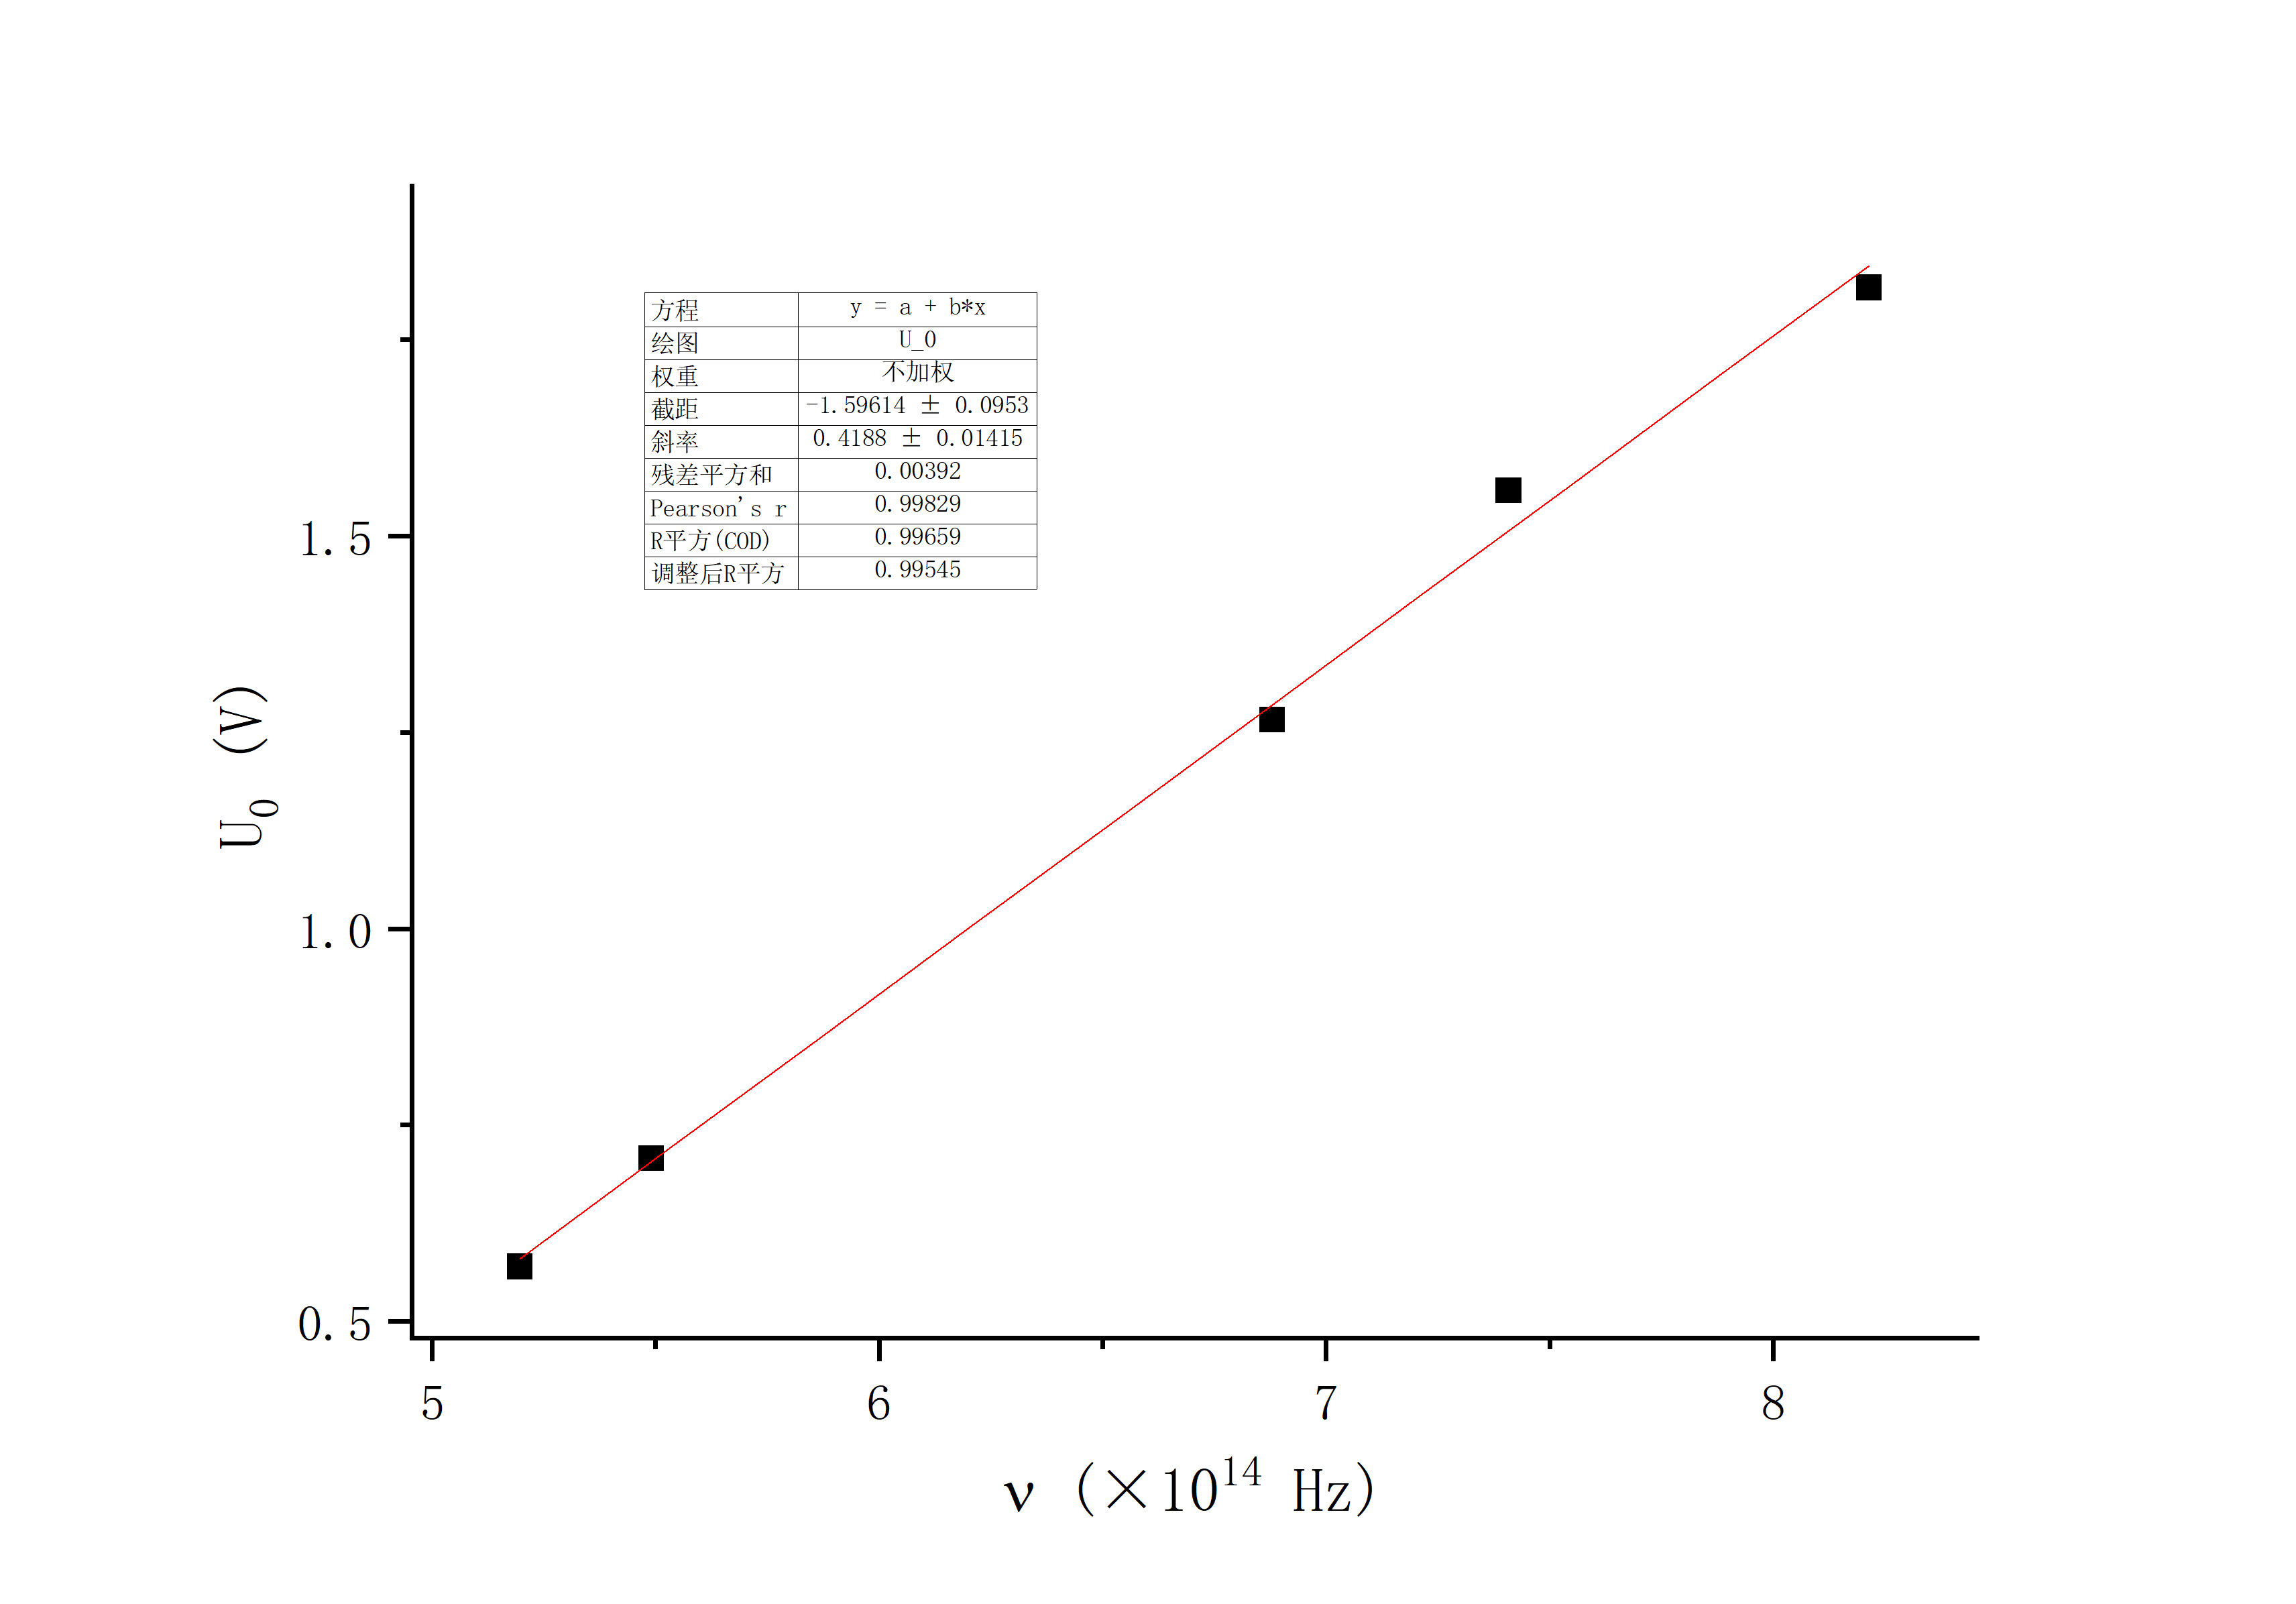
\includegraphics[width=0.8\linewidth]{1.png}
    \end{figure}
    拟合得到斜率为 0.4188$\times10^{-14}$ V$\cdot$s ,截距为 -1.596 V ,相关系数为 0.99829 ,故普朗克常数$h$为:
    \begin{equation*}
        h = ke = 0.4188\times10^{-14} \times 1.602\times10^{-19} = 6.709\times10^{-34} \text{J$\cdot$s}
    \end{equation*}
    相对误差为:
    \begin{equation*}
        E = \frac{|h-h_0|}{h_0} = \frac{|6.709\times10^{-34} - 6.626\times10^{-34}|}{6.626\times10^{-34}} \times 100\% = 1.25\%
    \end{equation*}
    \subsection{补偿法}
    使用孔径 4 mm 的光阑,改变滤波片,测得遏止电压值如下:
    \begin{table}[H]
        \centering
        \caption{补偿法测量遏止电压值与频率的关系}
        \begin{tabular}{ccc}
            \toprule
            波长$\lambda$ (nm) & 频率 $\nu$ ($\times10^{14}$ Hz) & 遏止电压 $U_0$ (V)\\
            \midrule
            577.0 & 5.196 & 0.578\\
            546.1 & 5.490 & 0.714\\
            435.8 & 6.879 & 1.270\\
            404.7 & 7.408 & 1.566\\
            365.0 & 8.214 & 1.822\\
            \bottomrule
        \end{tabular}
    \end{table}
    拟合图像如下:
    \begin{figure}[H]
        \centering
        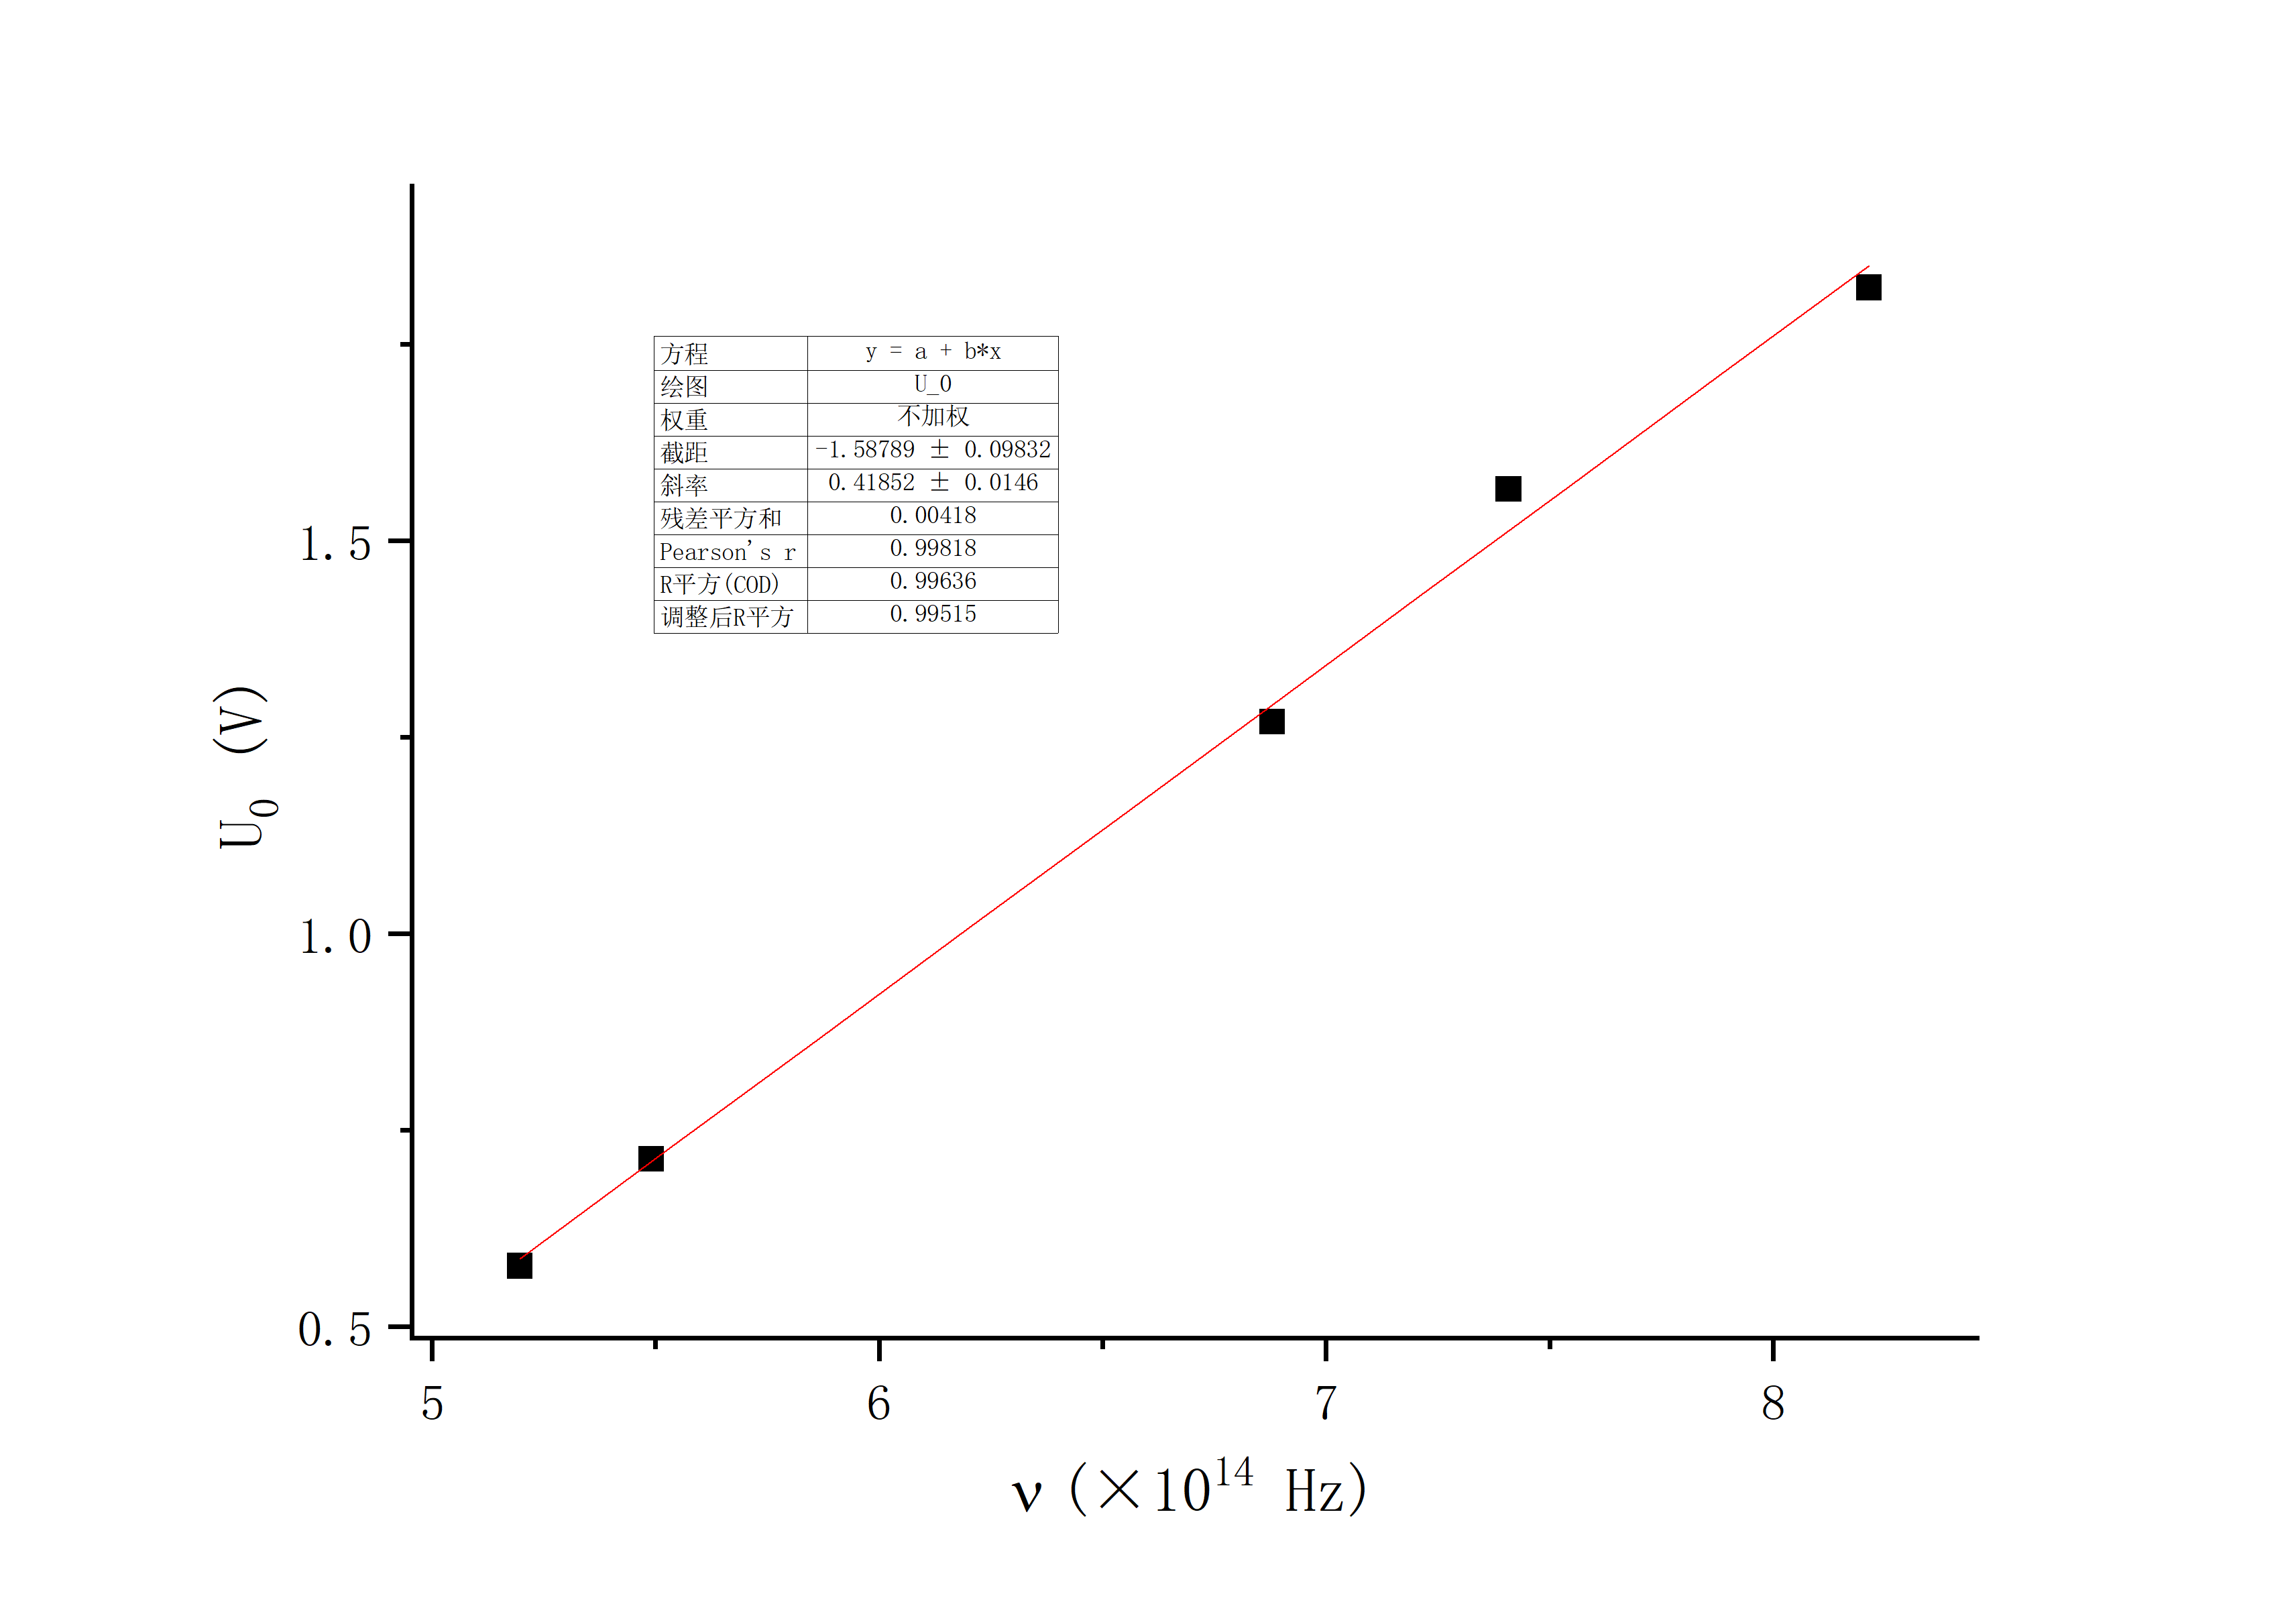
\includegraphics[width=0.8\linewidth]{2.png}
    \end{figure}
    拟合得到斜率为 0.4185$\times10^{-14}$ V$\cdot$s ,截距为 -1.588 V ,相关系数为 0.99818 ,故普朗克常数$h$为:
    \begin{equation*}
        h = ke = 0.4185\times10^{-14} \times 1.602\times10^{-19} = 6.704\times10^{-34} \text{J$\cdot$s}
    \end{equation*}
    相对误差为:
    \begin{equation*}
        E = \frac{|h-h_0|}{h_0} = \frac{|6.704\times10^{-34} - 6.626\times10^{-34}|}{6.626\times10^{-34}} \times 100\% = 1.18\%
    \end{equation*}
    光电管阴极材料的逸出功为:
    \begin{equation*}
        A = -be = 1.588 \text{eV}
    \end{equation*}
    光电管阴极材料的截止频率为:
    \begin{equation*}
        \nu_0 = \frac{A}{h} = \frac{1.588\times1.602\times10^{-19}}{6.704\times10^{-34}} = 3.79\times10^{14} \text{Hz}
    \end{equation*}
    \section{饱和光电流与光强的关系}
    \subsection{通过改变孔径改变光强}
    \subsubsection{波长为 435.8 nm}
    设置电压为30 V ,测得光电流数据如下:
    \begin{table}[H]
        \centering
        \caption{波长为 435.8 nm 时光电流与孔径的关系}
        \begin{tabular}{cc}
            \toprule
            孔径 $\Phi$ (mm) & 光电流 $I$ ($\times10^{-10}$A)\\
            \midrule
            2 & 7.0\\
            4 & 25.4\\
            8 & 100.9\\
            14.35 & 304\\
            \bottomrule
        \end{tabular}
    \end{table}
    光电流与孔径的平方呈线性关系,拟合图像如下:
    \begin{figure}[H]
        \centering
        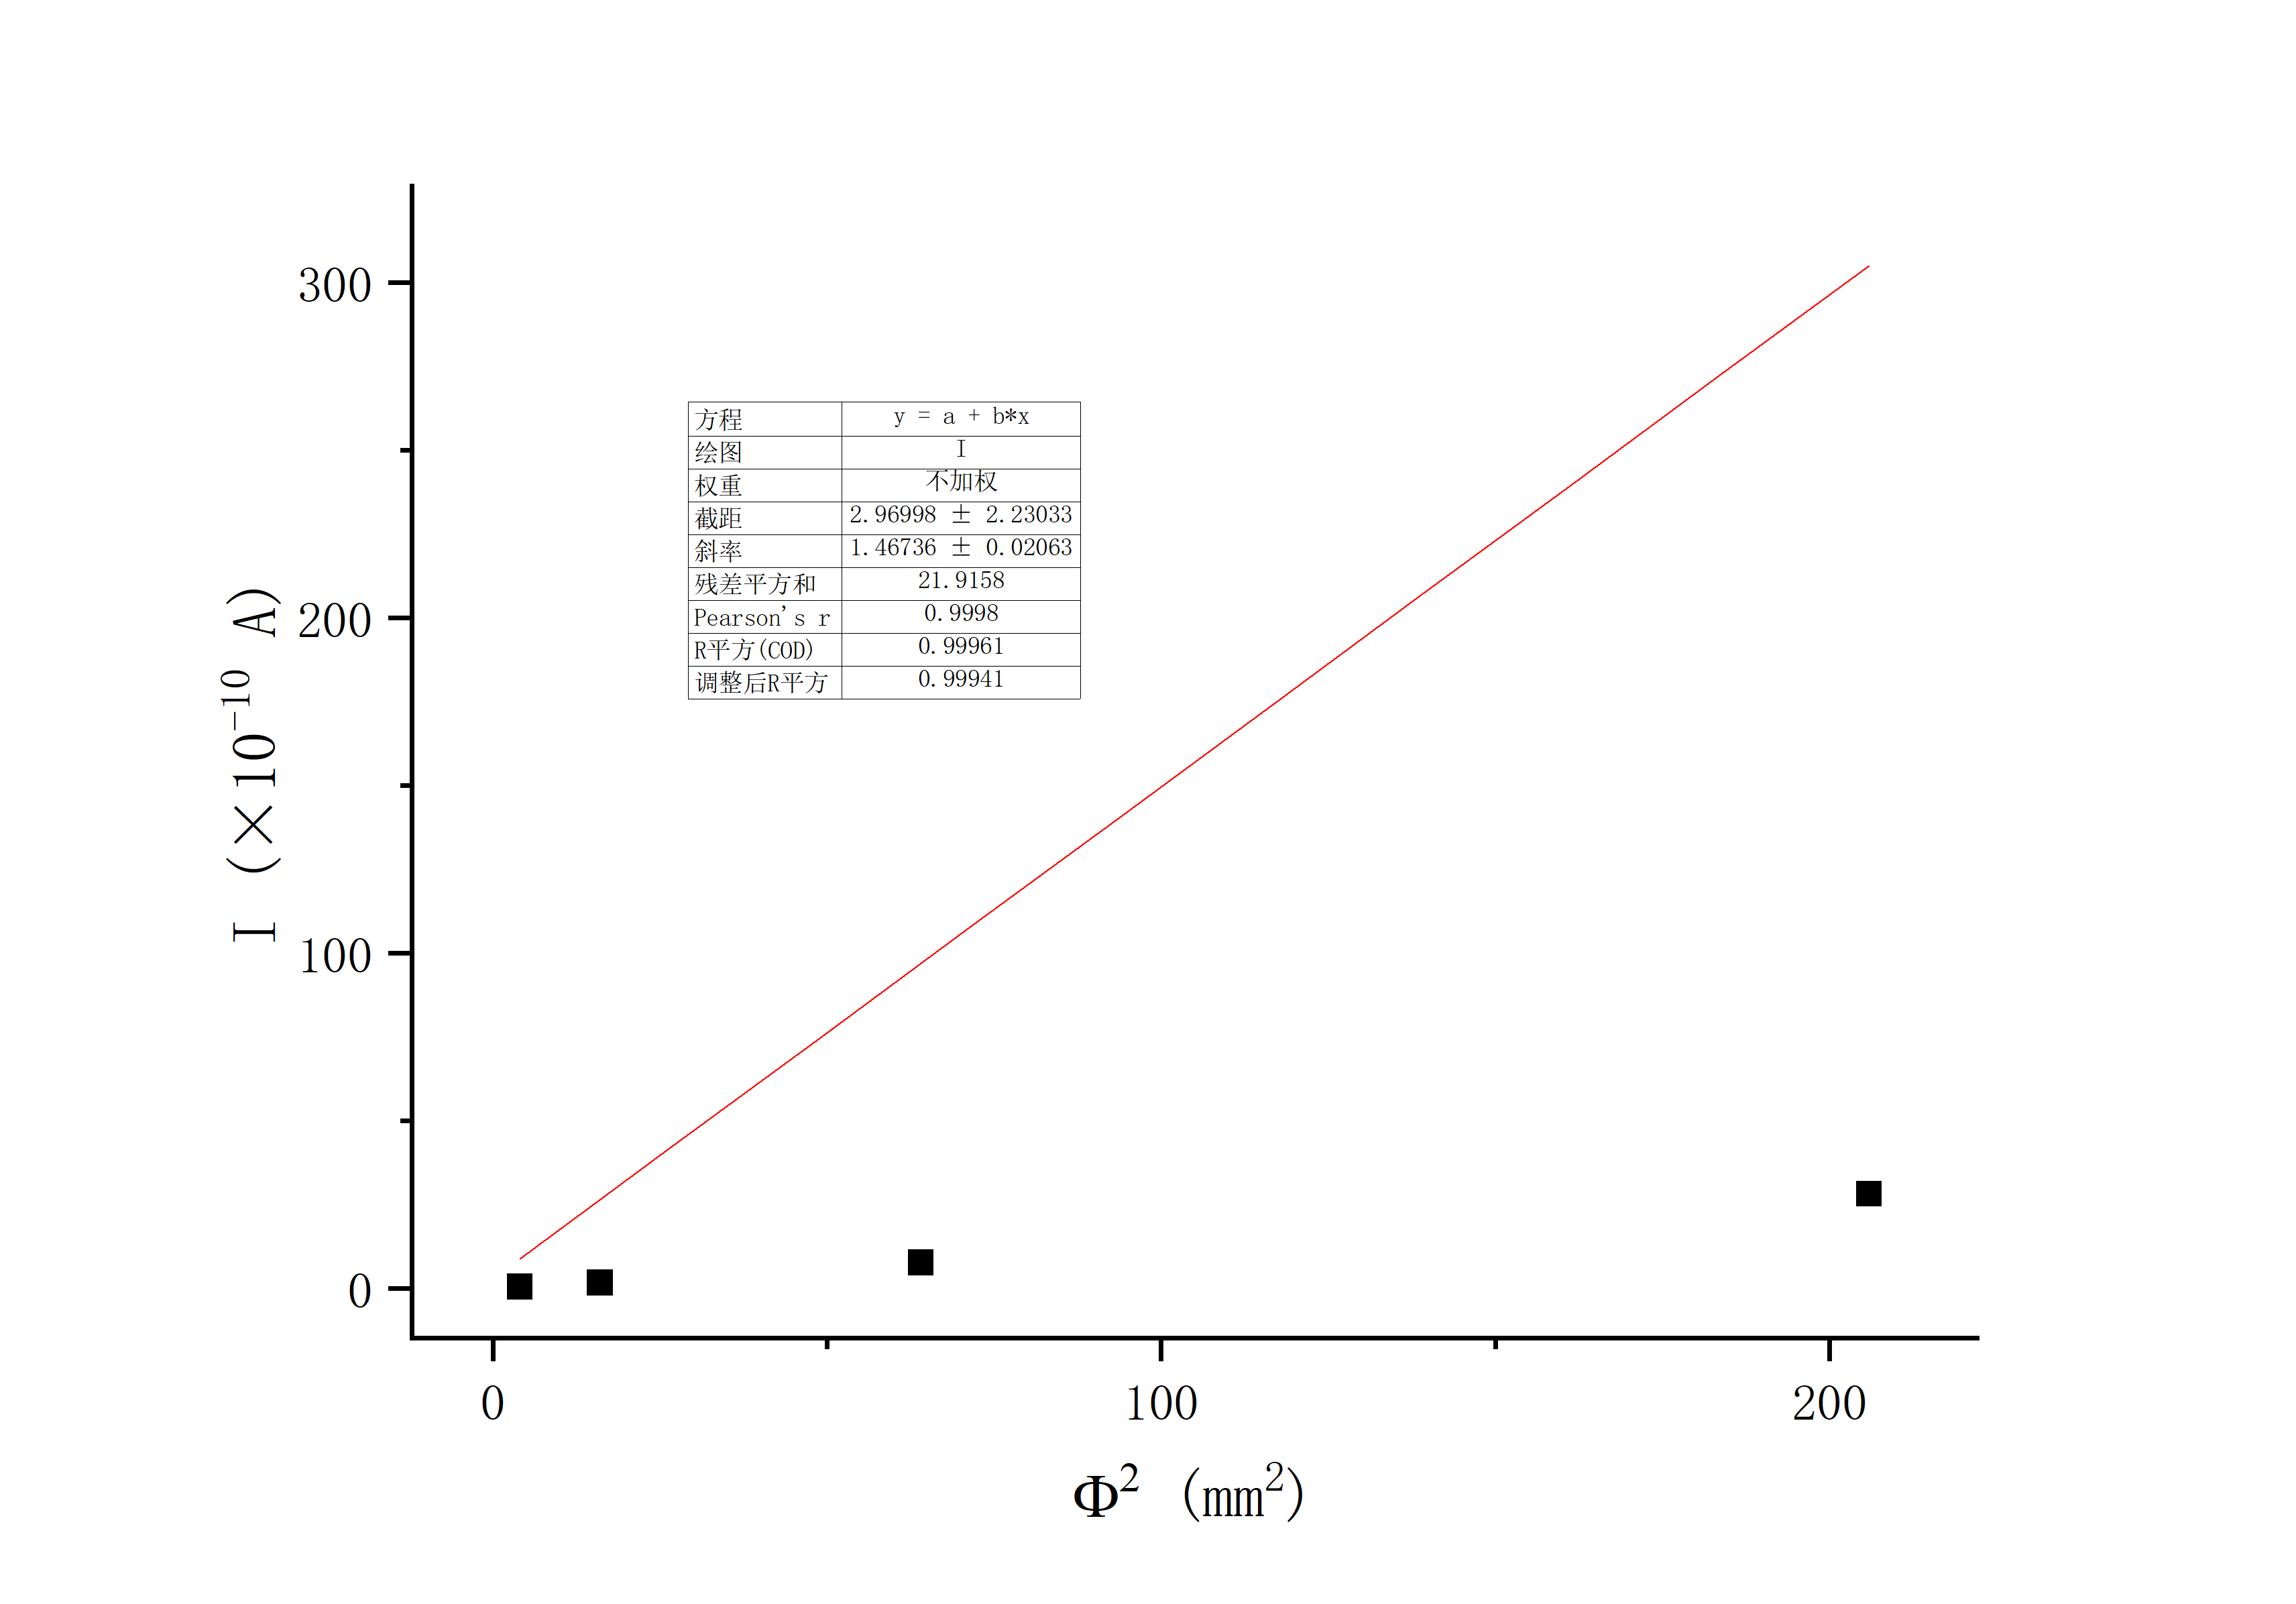
\includegraphics[width=0.8\linewidth]{3.png}
    \end{figure}
    拟合得到斜率为 1.467 A/mm$^2$ ,截距为 2.970$\times10^{-10}$ A ,相关系数为 0.9998 。
    \subsubsection{波长为 546.1 nm}
    设置电压为30 V ,测得光电流数据如下:
    \begin{table}[H]
        \centering
        \caption{波长为 546.1 nm 时光电流与孔径的关系}
        \begin{tabular}{cc}
            \toprule
            孔径 $\Phi$ (mm) & 光电流 $I$ ($\times10^{-10}$A)\\
            \midrule
            2 & 0.5\\
            4 & 1.7\\
            8 & 7.7\\
            14.35 & 28.2\\
            \bottomrule
        \end{tabular}
    \end{table}
    光电流与孔径的平方呈线性关系,拟合图像如下:
    \begin{figure}[H]
        \centering
        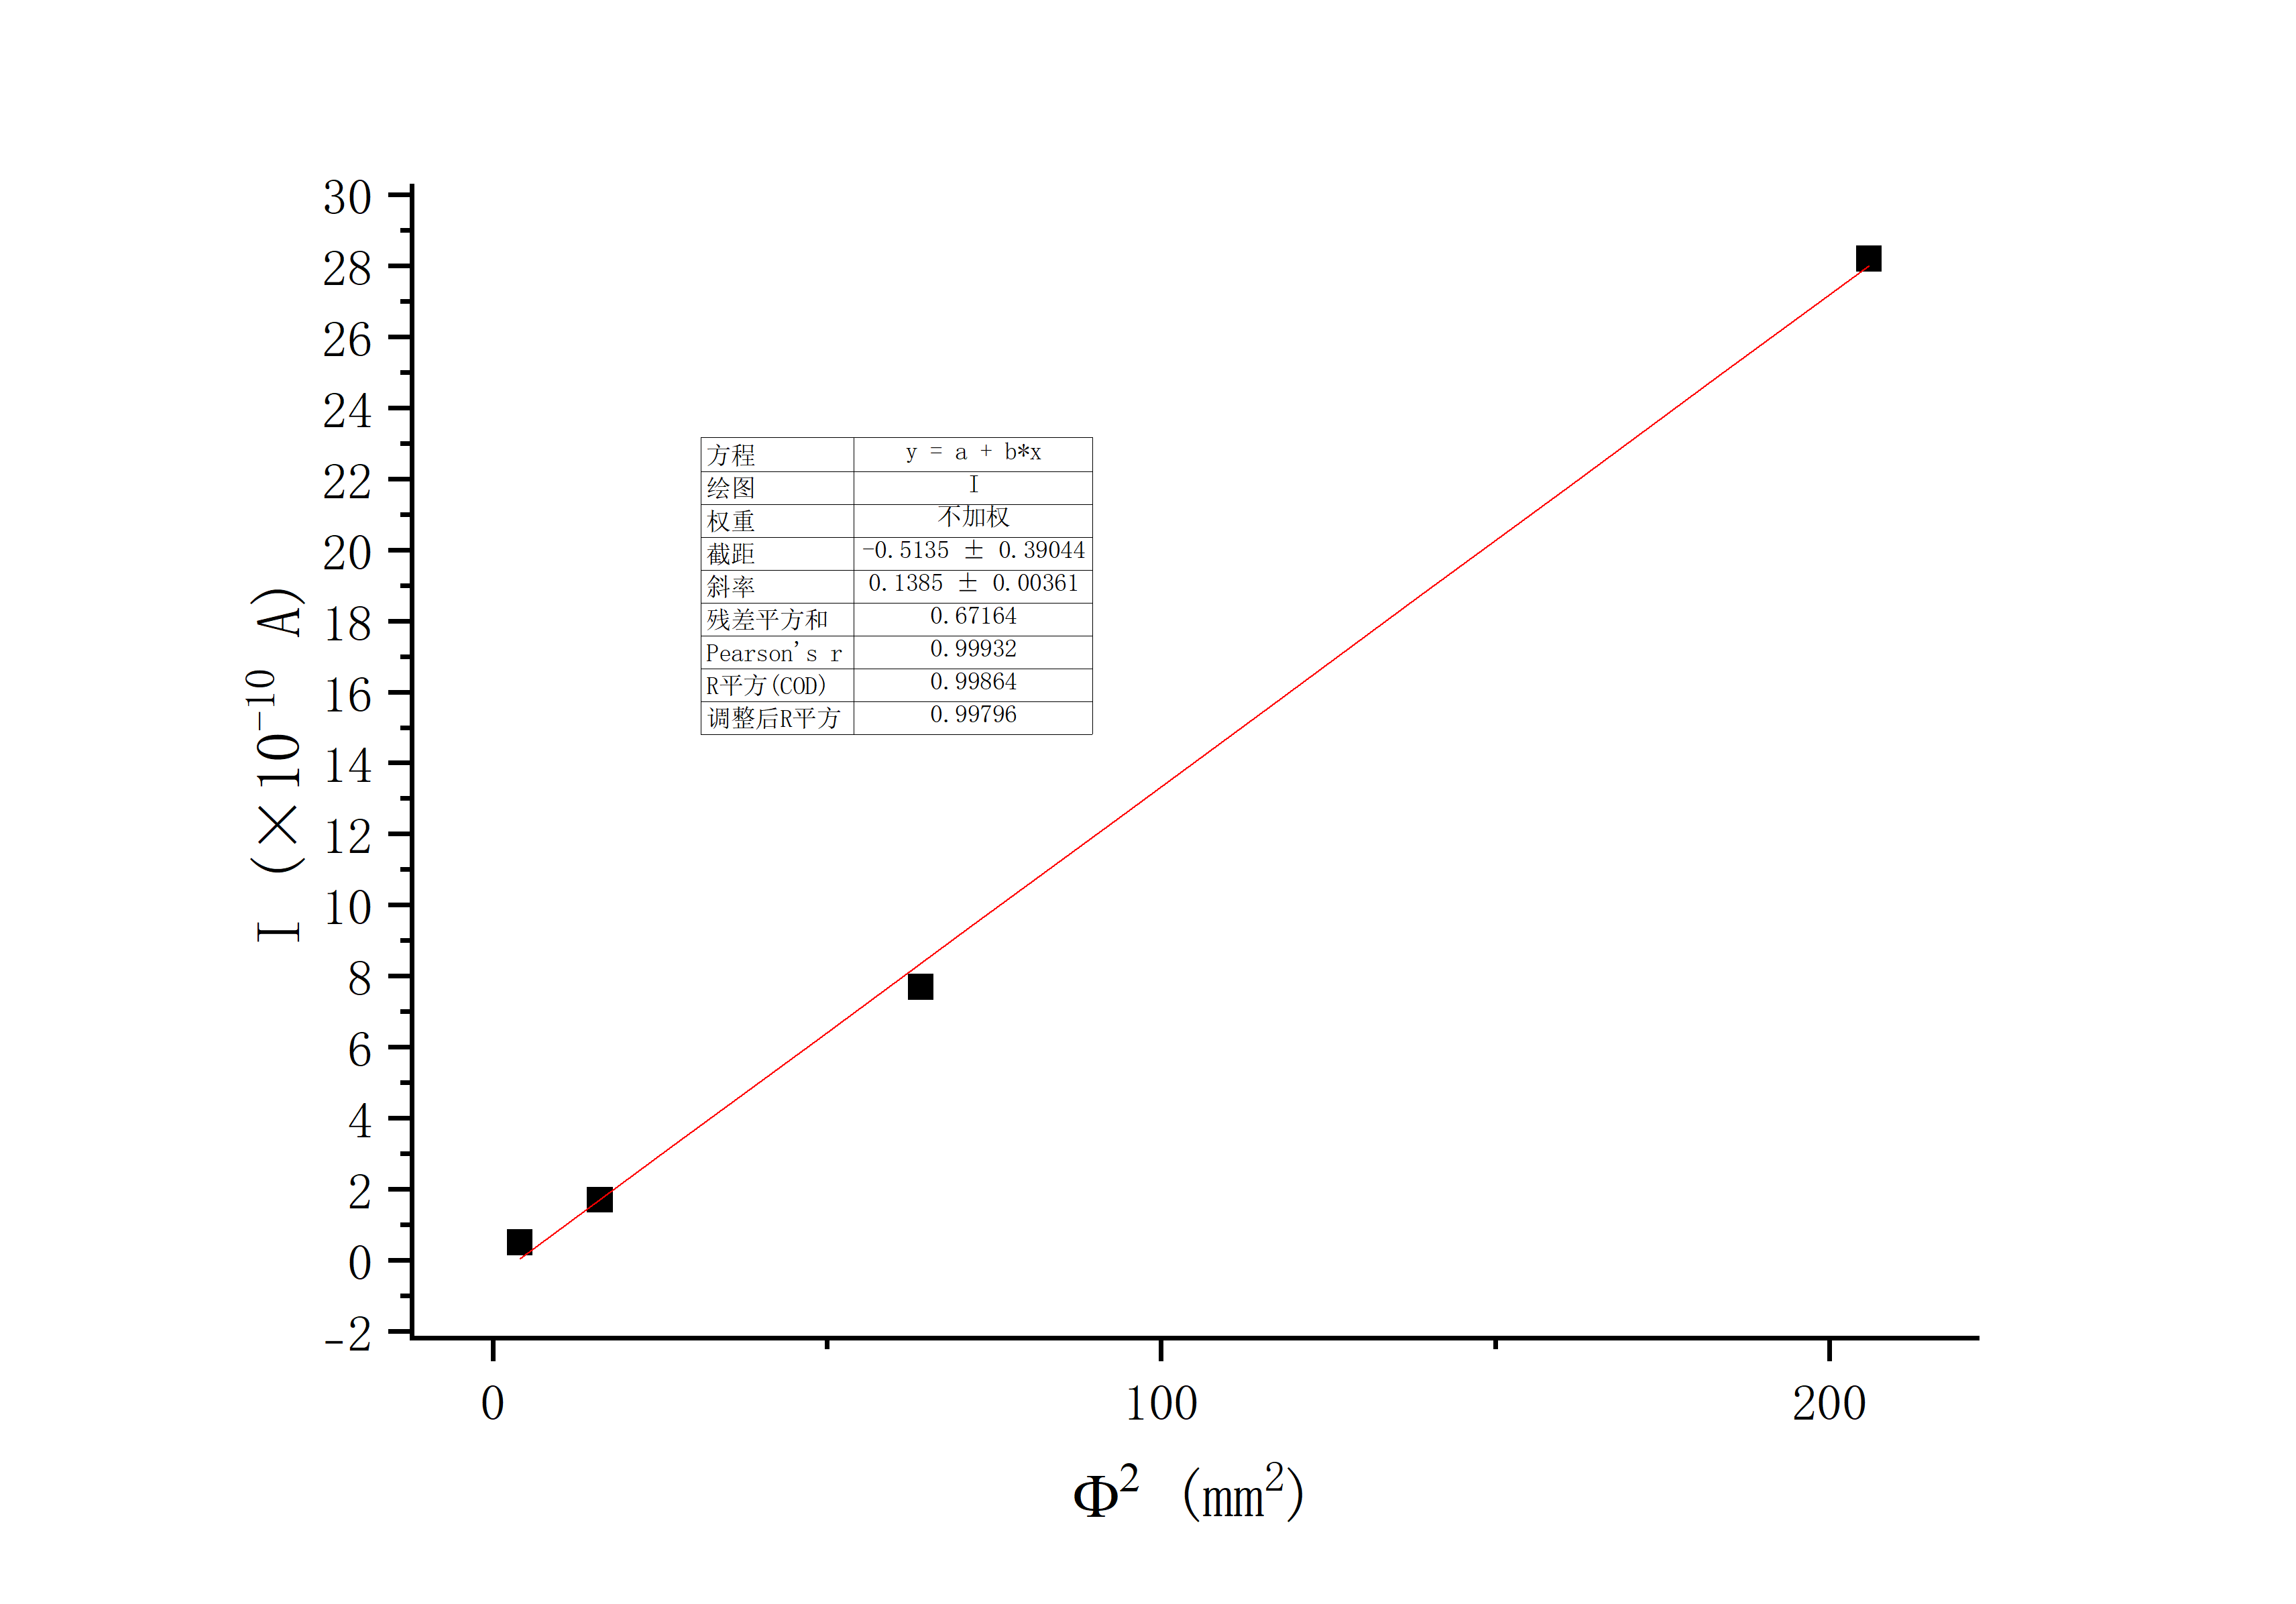
\includegraphics[width=0.8\linewidth]{4.png}
    \end{figure}
    拟合得到斜率为 0.1385 A/mm$^2$ ,截距为 -0.5135$\times10^{-10}$ A ,相关系数为 0.9993 。
    \subsection{通过改变距离改变光强}
    \subsubsection{波长为 435.8 nm}
    设置电压为30 V ,改变光电管和光源之间距离,测得光电流数据如下:
    \begin{table}[H]
        \centering
        \caption{波长为 435.8 nm 时光电流与距离的关系}
        \begin{tabular}{cc}
            \toprule
            距离 $d$ (cm) & 光电流 $I$ ($\times10^{-10}$A)\\
            \midrule
            40 & 25.3\\
            38 & 28.9\\
            36 & 32.8\\
            34 & 38.8\\
            32 & 46.5\\
            30 & 55.7\\
            \bottomrule
        \end{tabular}
    \end{table}
    光强与距离的平方成反比关系,拟合图像如下:
    \begin{figure}[H]
        \centering
        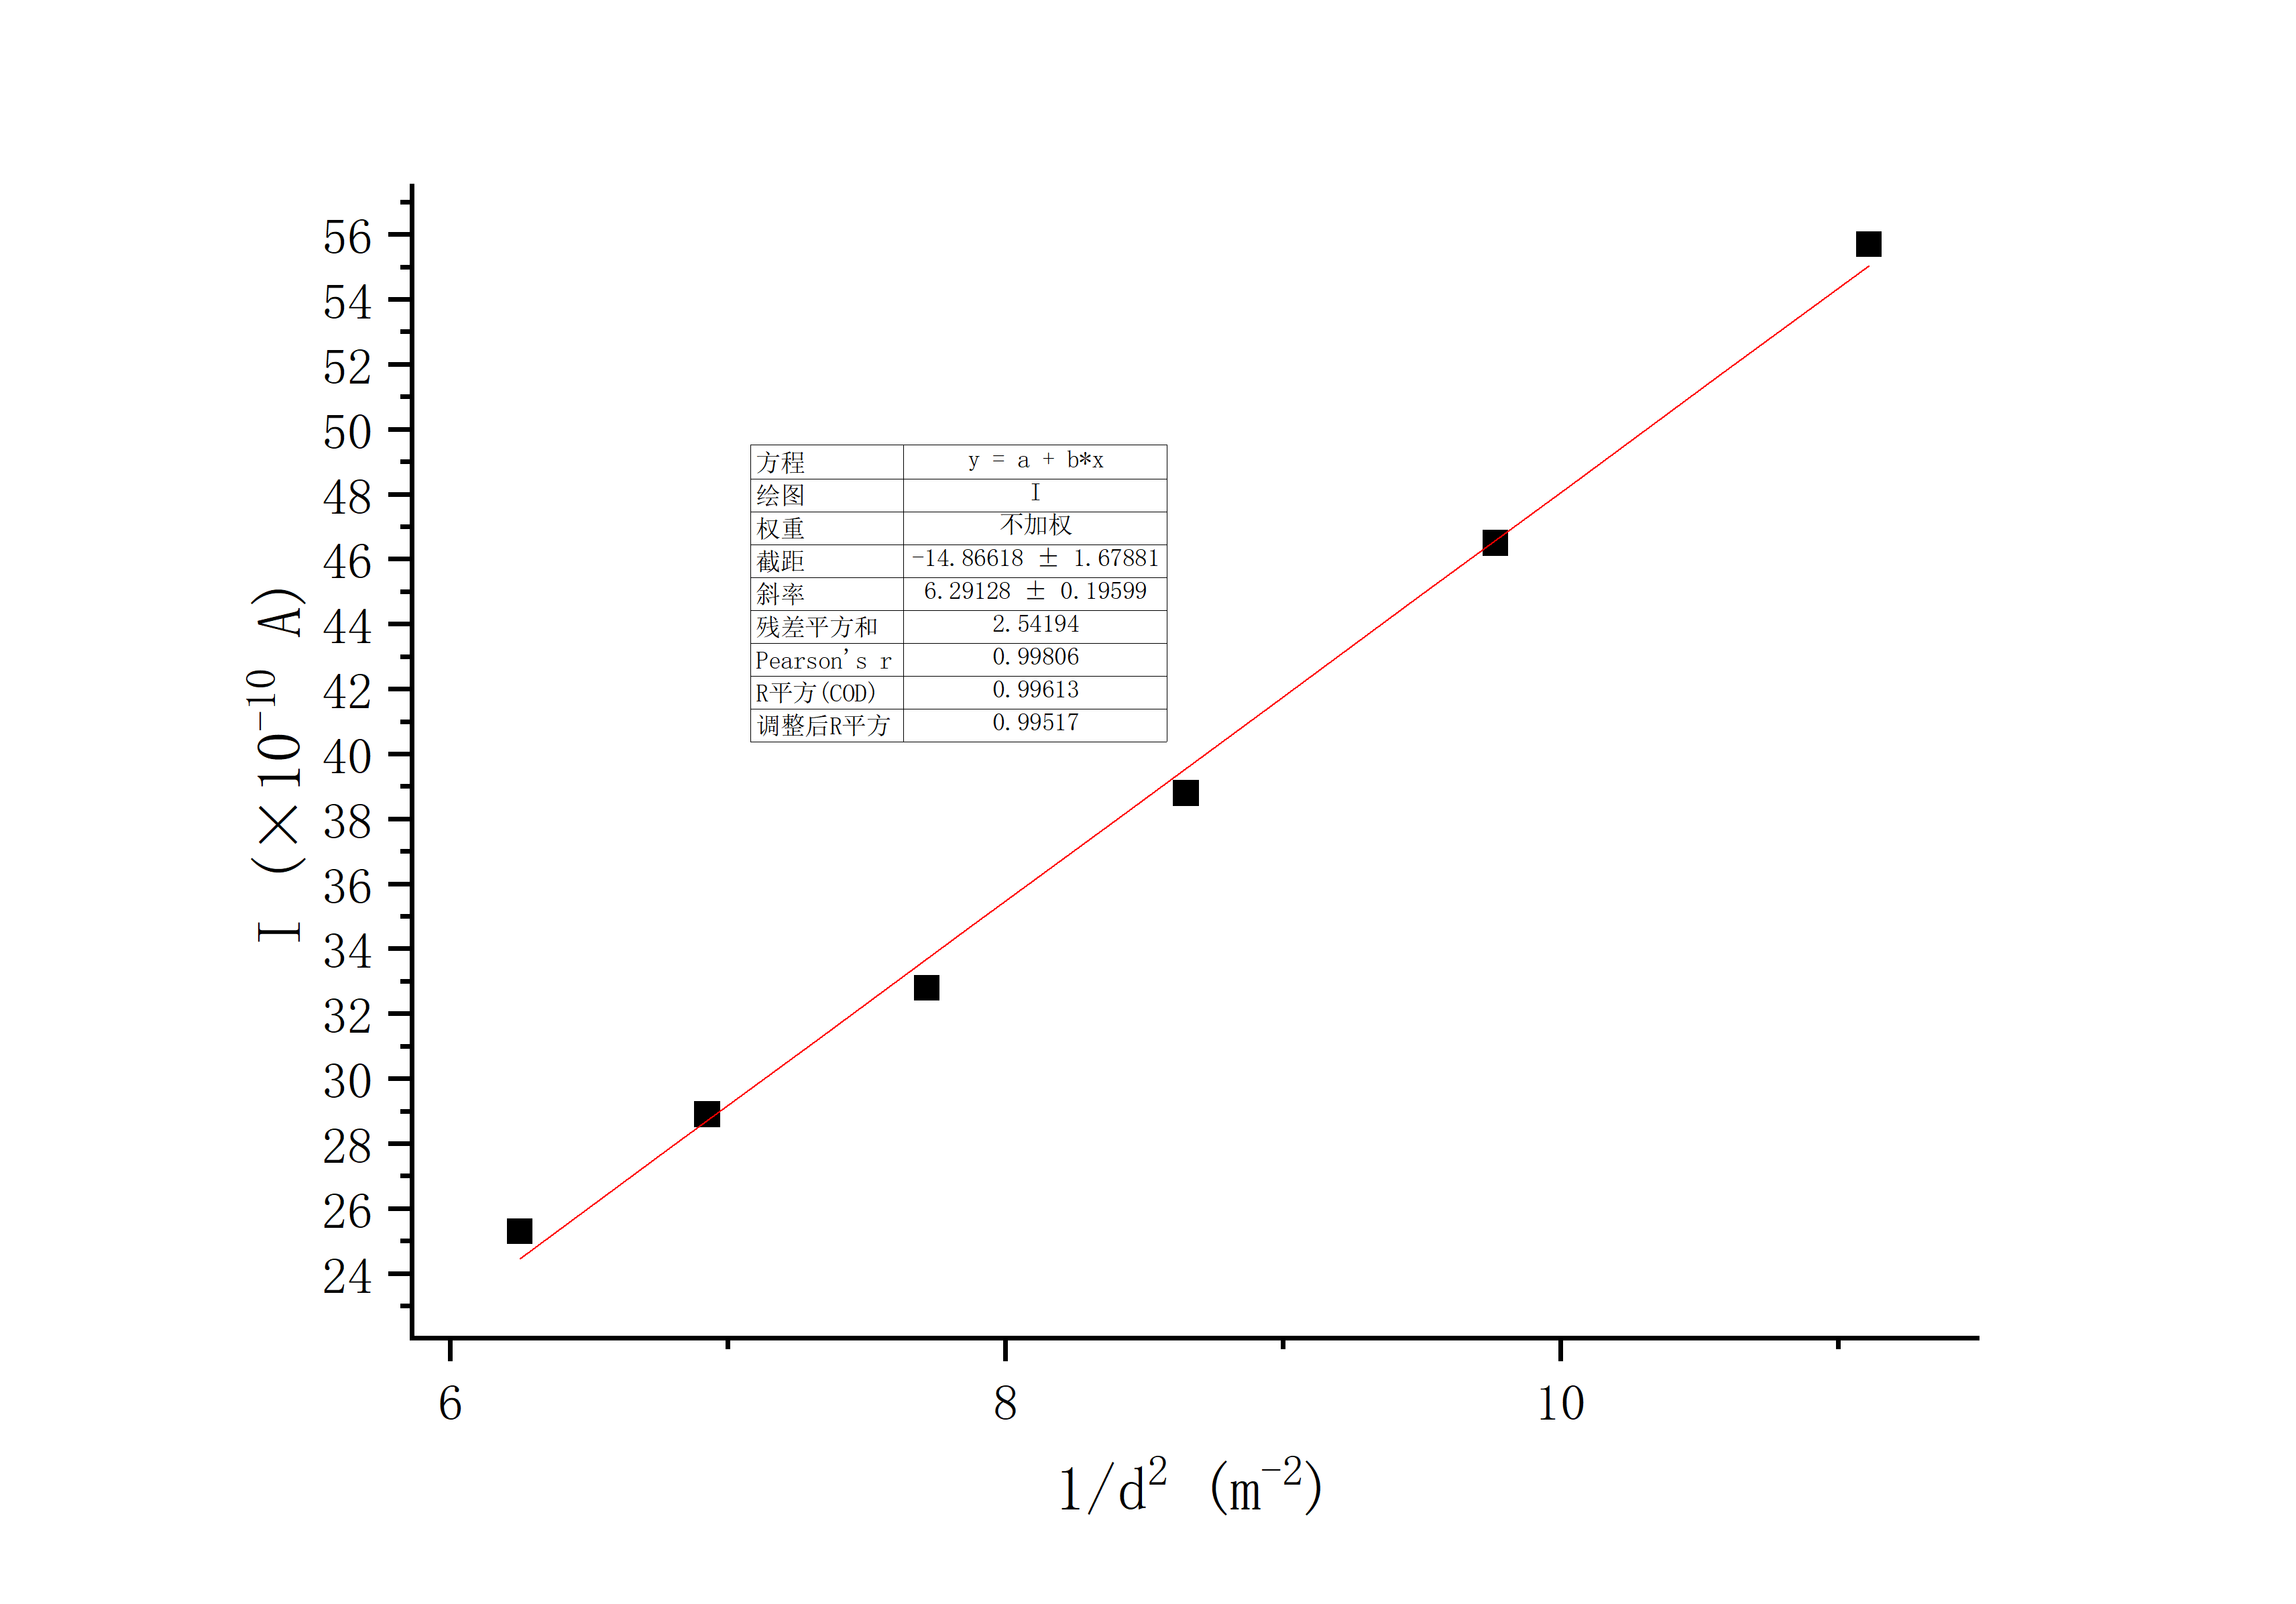
\includegraphics[width=0.8\linewidth]{5.png}
    \end{figure}
    拟合得到斜率为 6.291$\times10^{-10}$ A$\cdot$m$^2$ ,截距为 -14.87$\times10^{-10}$ A ,相关系数为 0.9981 。
    \subsubsection{波长为 546.1 nm}
    设置电压为30 V ,改变光电管和光源之间距离,测得光电流数据如下:
    \begin{table}[H]
        \centering
        \caption{波长为 546.1 nm 时光电流与距离的关系}
        \begin{tabular}{cc}
            \toprule
            距离 $d$ (cm) & 光电流 $I$ ($\times10^{-11}$A)\\
            \midrule
            40 & 16.7\\
            38 & 19.0\\
            36 & 22.8\\
            34 & 27.1\\
            32 & 32.7\\
            30 & 40.7\\
            \bottomrule
        \end{tabular}
    \end{table}
    光强与距离的平方成反比关系,拟合图像如下:
    \begin{figure}[H]
        \centering
        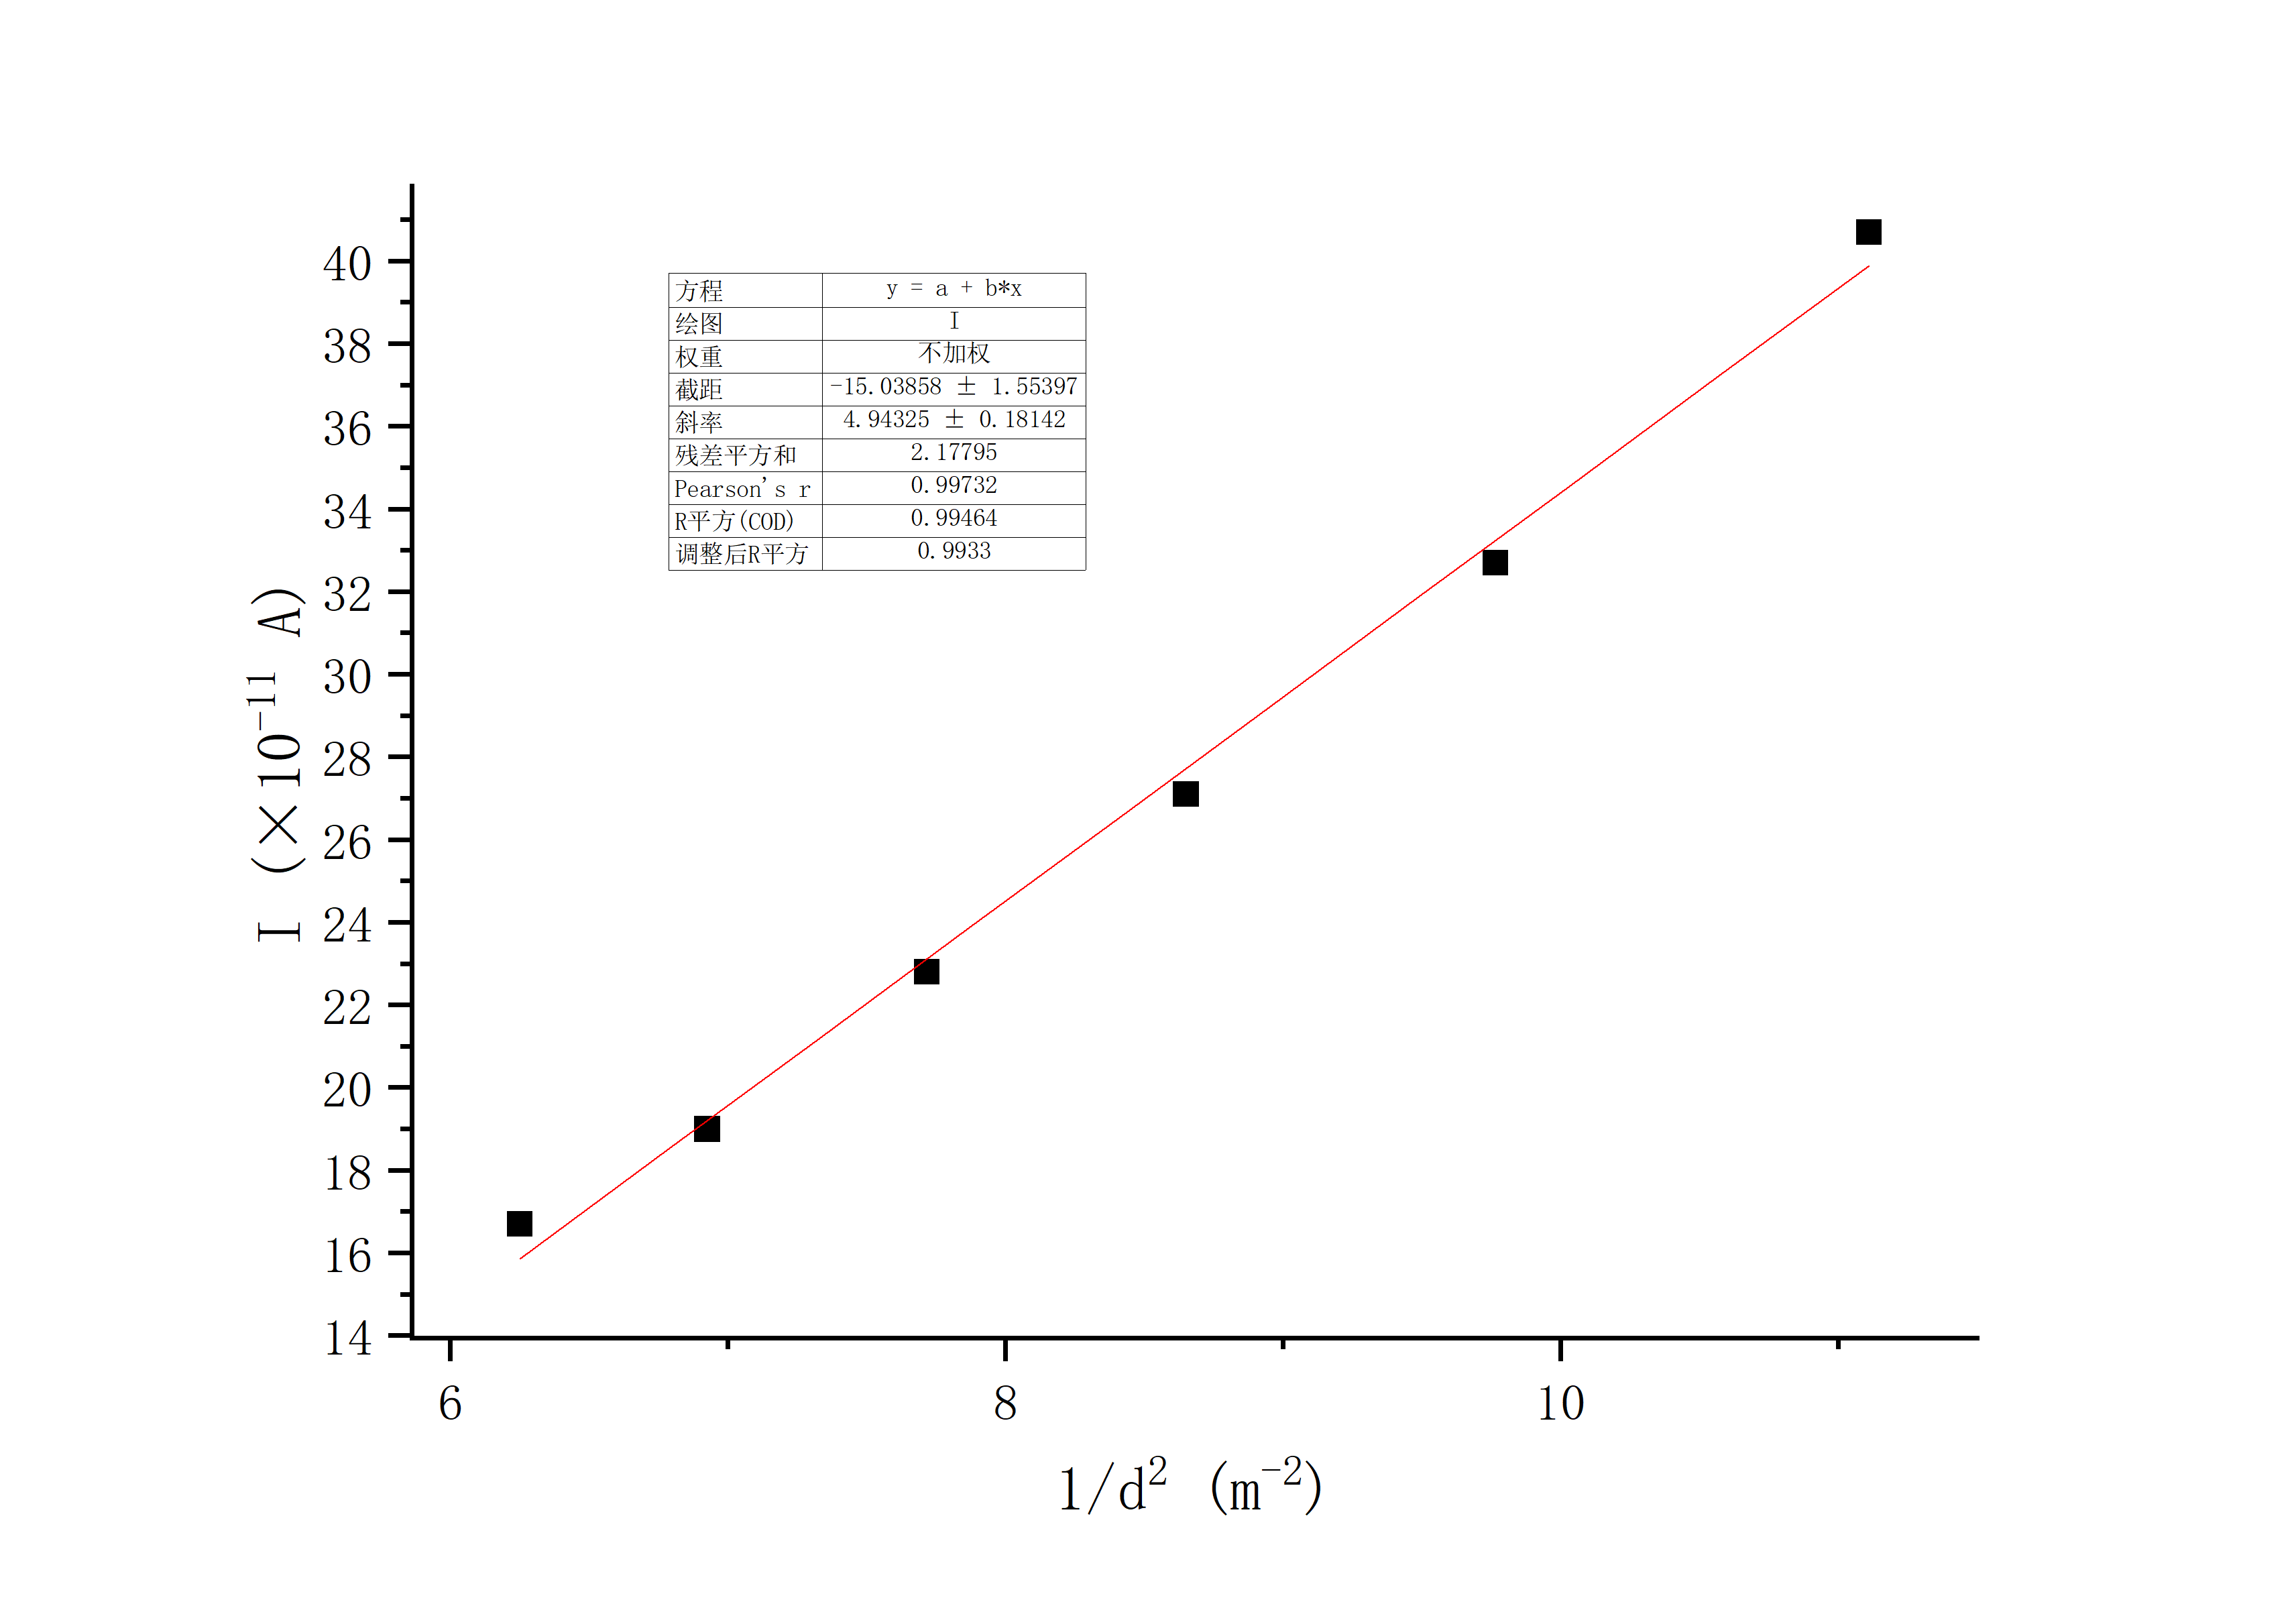
\includegraphics[width=0.8\linewidth]{6.png}
    \end{figure}
    拟合得到斜率为 4.943$\times10^{-11}$ A$\cdot$m$^2$ ,截距为 -15.04$\times10^{-11}$ A ,相关系数为 0.9973 。
    \newpage
    \section*{附录}
    老师签字的实验数据:
    \begin{figure}[H]
        \centering
        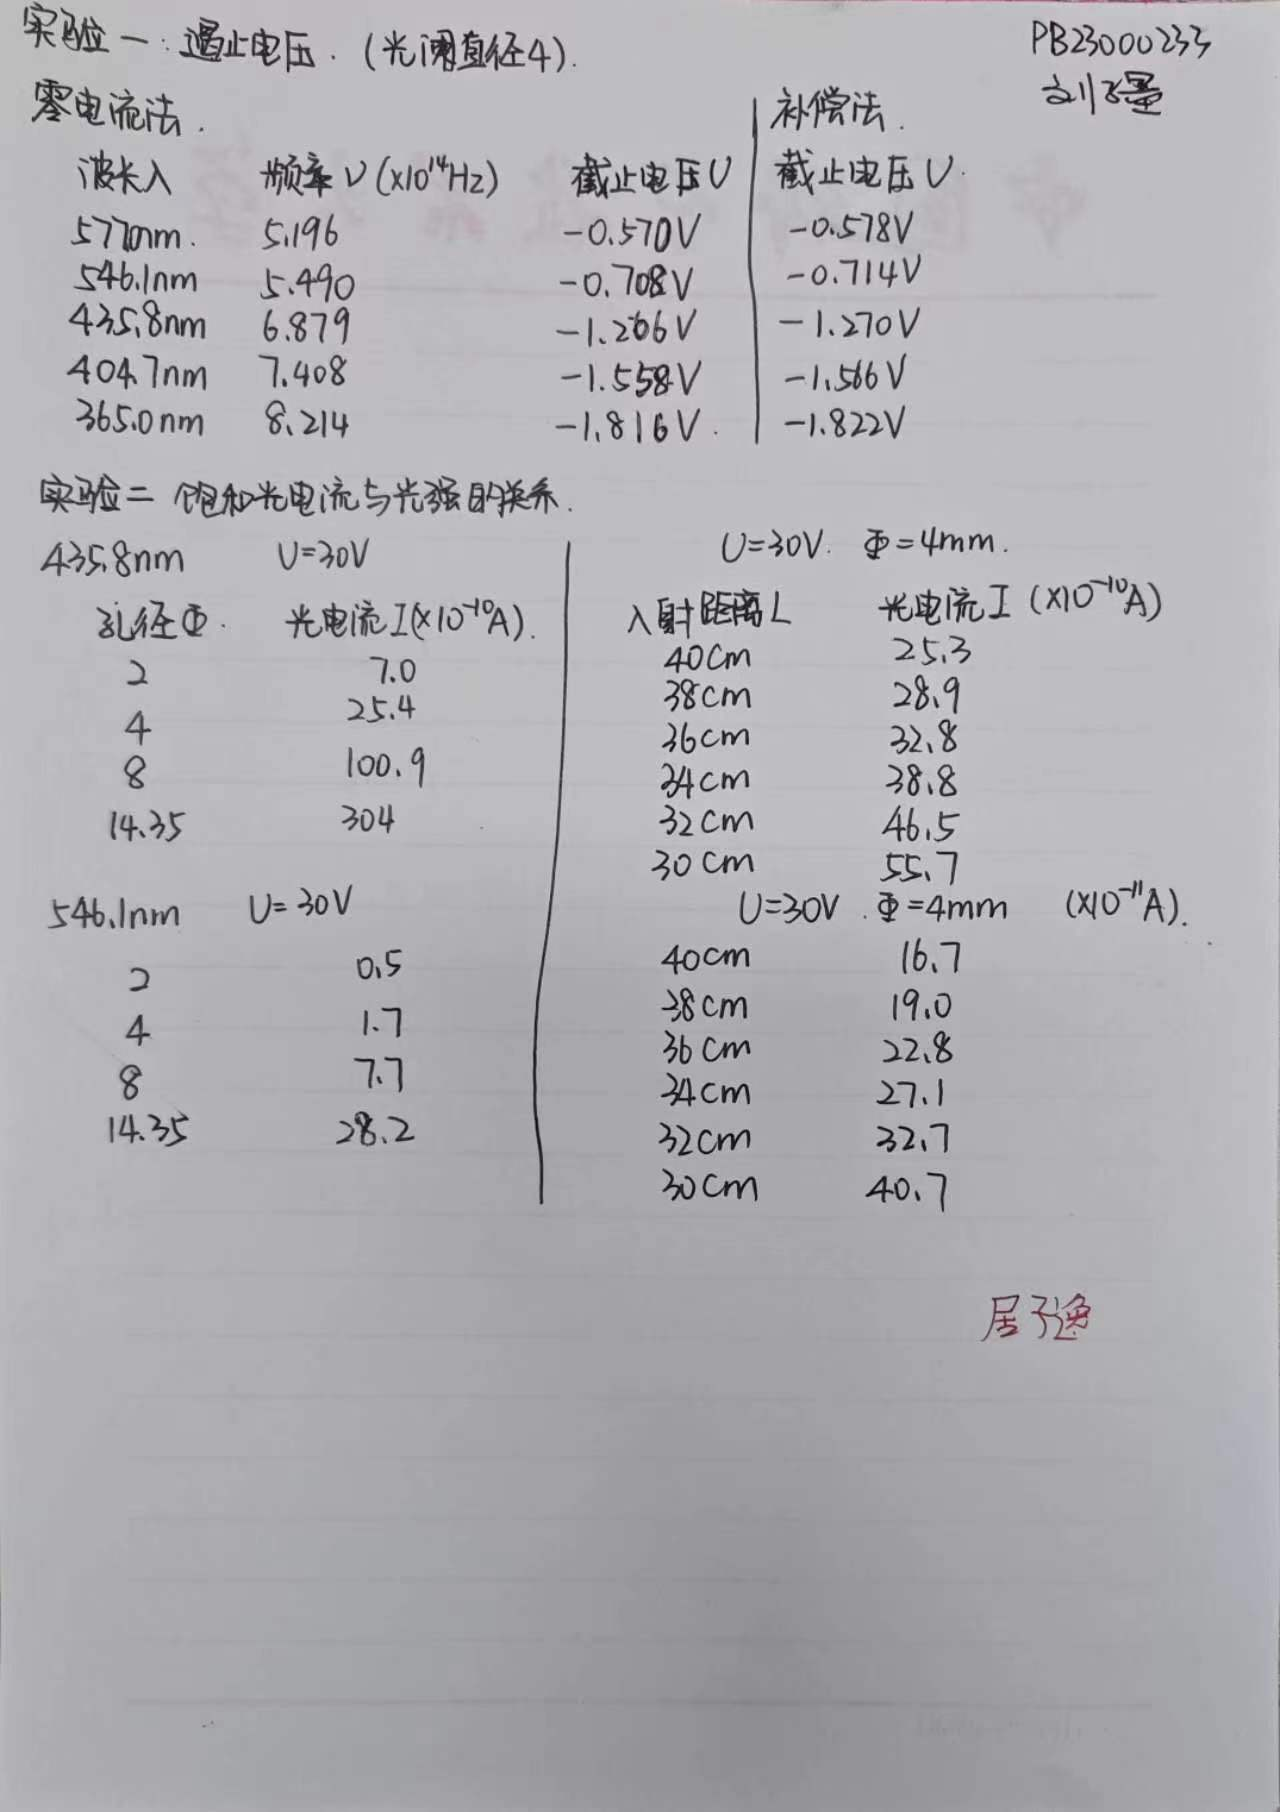
\includegraphics[width=0.98\linewidth]{shuju.jpg}
    \end{figure}
\end{document}
